Descriviamo in questa sezione le tecnologie che sono state scelte per la realizzazione di Nexify.\\
Per la CDN è stato scelto Amazon CloudFront, che ha dimostrato con altre piattaforme di essere in grado di scalare a livello mondiale e fornisce costi che dipendono dal consumo effettuato. In realtà CloudFront sarà affiancato da altri servizi Amazon, e in particolare verrà adottata l'architettura di video streaming on demand proposta da Amazon:\\
\begin{figure}[!h]
\centering
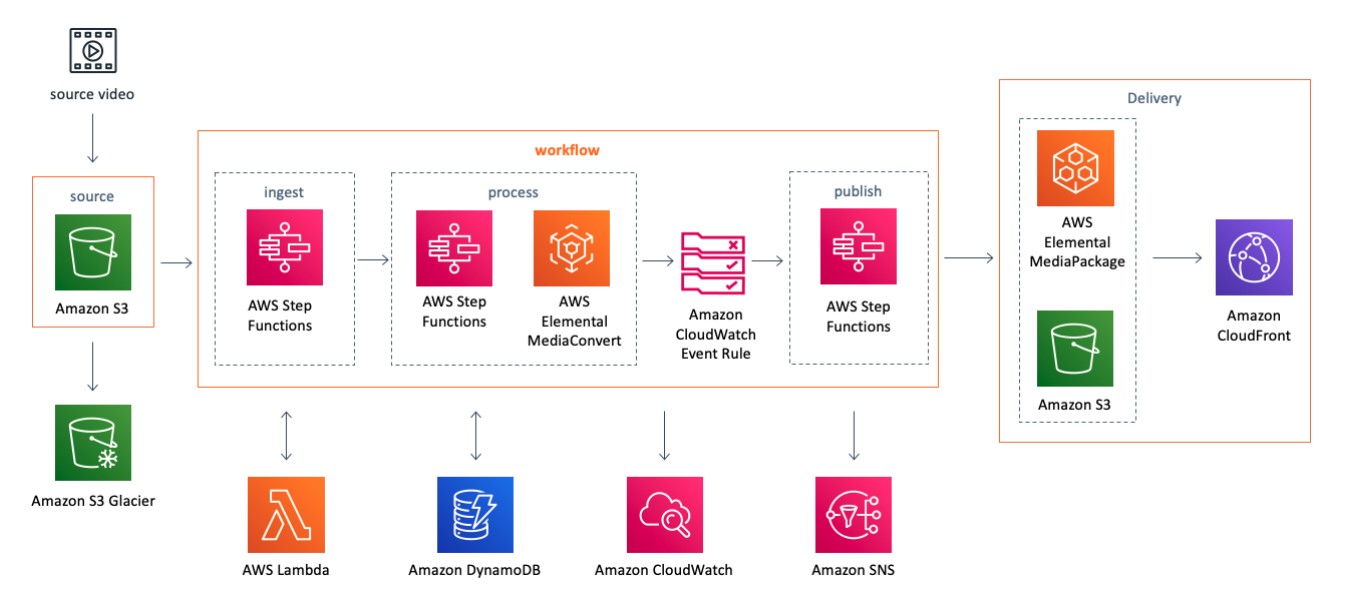
\includegraphics[scale=0.45]{aws_ondemand_streaming.png}
\end{figure}\\
Quando un utente carica un video, questo viene memorizzato usando Amazon S3, che è un servizio di storage di oggetti. Si entra poi in una fase di ingest in cui vengono fatti controlli sul corretto caricamento del file, sul formato del file e controlli simili; una volta superati questi controlli si entra nella fase di process in cui si creano varie versioni del video codificate in formati diversi in modo da garantire la disponibilità su una vasta gamma di dispositivi, le versioni avranno anche bitrate diversi in modo da poter effettuare uno streaming adattivo. Viene poi genarato un URL per il video su S3 e CloudFront, con il quale è possibile accedere al video. L'architettura fornisce anche altre funzionalità, come Simple Notification Service che invia notifiche all'amministratore in casi di errore, il database Dynamo viene usato, tra le altre cose, per tenere un log delle operazioni eseguite nell'infrastruttura. CloudFront è la CDN vera e propria, a cui gli utenti faranno richieste per ricevere video in streaming, AWS Elemental Media Package è utile per preparare i dati allo streaming e consente facilmente di gestire operazioni quali la pausa dello streaming e lo spostamento del punto di riproduzione.
\newline\newline
\noindent{\large \textbf{Revisioni 11}} \\ \\
\begin{tabular}{|c | c | c | c|} 
 	\hline
	 Numero & Data & Descrizione \\ [0.5ex] 
	\hline\hline
	1 & 20/04/2020 & Stesura iniziale \\ 
	\hline
\end{tabular}